\documentclass{article}
\usepackage{amsmath,amssymb,url}
\usepackage{graphicx}
\usepackage[table,x11names]{xcolor}
\usepackage{float}



\author{Brad Schoenrock\\Video Operations Engineering\\Charter Communications\\Greenwood Village, CO}
\title{AV2.11 to AV2.16 Stitcher/Session Memory Use - BODCMA\\Charter Internal Note.\\Draft Version 1.0.0}
\date{Dec. 2019}
\begin{document}
\maketitle
\newpage

\tableofcontents
\newpage

\section{Introduction}
\label{SECTION-Introduction}

Session Size analysis was performed in AV2.11, which showed memory usage to be significantly higher than was expected. AV2.16 brings changes to webkit, which are expected to bring the largest sessions down in size due to improvements to the garbage collector which deallocates memory which is no longer in use. Further improvments are expected with the delivery of SGUI's NNS project. With these performance improvements underway, this document serves as a first look into the performance provided by the switch to Webkit-V3 bundled in the deployment of AV2.16 in Boston. 

\section{RSS vs. SIZE}
\label{SECTION-RSS}

The Resident Set Size(RSS) of a process in linux is a measure of memory used, but does not include memory which is swapped out, or memory which is being used in shared memory libraries. Virtual Memory Size (VMS) aka SIZE includes all memory the process can access, including swap memory and memory which has been alocated but not used. This means that RSS under-reports memory used, while VMS over-reports memory used. In AV2.16 VMS has become unusable for capacity planning because of how memory is allocated in webkit-V3. RSS in AV2.16. Linux reports that RSS used by a webkit process may be 250MB, while the VMS is allocating 100GB per session on Boston's stitchers that only have 128GB of memory. There are three usual causes for large virtual memory utalization which don't materialize into real memory usage. Those are extensive use of swap memory, use of large shared libraries, and memory which is allocated to the buffer/cache but is not used. A 'free -m' command reveals no use of swap memory, some use of shared memory, but does show up as a significant allocation to buffer/cache memory. This means that most of that VMS memory is allocated but not used. Some shared memory libraries are being used, but not at the level to explain the VMS reported size of each process. A better understanding of how webkit manages its memory allocations and shared memory will be nessicary going forward to ensure accurate capacity planning can be acomplished in AV2.16+ environments. 



\section{Memory Consumption AV2.11}
\label{SECTION-211Memory}


The memory utilization of the html5client process on the Boston stitchers in AV2.11 is summarized in table~\ref{TABLE-AV211SessionSize}. Here we can see the difference between RSS and VMS reported by linux. The average AV2.11 session is using 460MB of memory when reported by RSS, and 744 MB of memory when reported by SIZE (VMS). This difference comes down to buffer/cache memory and shared memory utalization in the webkit-V2 environment. It is worth noting that the largest session in Boston at the time of measurement was 1.6GB RSS which corresponds to 2.0GB VMS. The memory use can be visualized in figure~\ref{FIGURE-AV211SessionSize} and figure~\ref{FIGURE-AV211SizeVsTime}. CPU use can be seen in figure~\ref{FIGURE-AV211CPUVsTime}.



\begin{table}[H]
\begin{tabular}{|l|l|l|l|l|}
\hline BODCMA&        ELAPSED&        CPU\%&      RSS(mb)&     SIZE(mb) \\
\hline count&                     874&  874&   874&   874 \\
\hline mean&   0 days 00:39:06&    5.614&   460.363&   744.067 \\
\hline std&    0 days 00:54:03&   12.516&   235.365&   356.619 \\
\hline min&           0 days 00:00:00&    0.000&    45.016&    89.824 \\
\hline 25\%&    0 days 00:02:41&    0.300&   280.316&   461.015 \\
\hline 50\%&           0 days 00:20:01&    0.800&   343.302&   555.522 \\
\hline 75\%&    0 days 00:54:59&    4.800&   625.310&  1066.030 \\
\hline max&           0 days 07:49:03&  102.000&  1612.384&  2080.036 \\
\hline 
\end{tabular}
\caption{\label{TABLE-AV211SessionSize}Size of the html5client in AV2.11 from BODCMA on 12/10.} 
\end{table}



\begin{figure}[H]
        \center{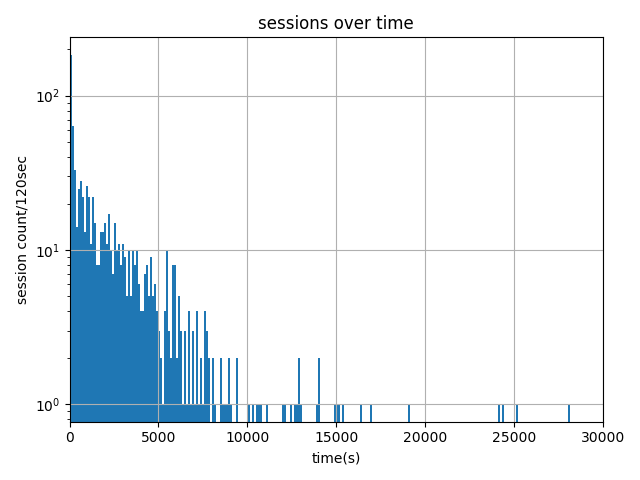
\includegraphics[width=\textwidth]
        {figures/211SessionLength}}
        \caption{\label{FIGURE-AV211SessionSize} Histogram of session size over lifetime of session in AV2.11. Note: the 0-2min bin is not visible in this rendering, but there are 184 sessions under 2 min duration. Note: logarithmic scale on Y axis. Note: longest running session is 7 hrs 49 min which is a valid session.}
\end{figure}

\begin{figure}[H]
        \center{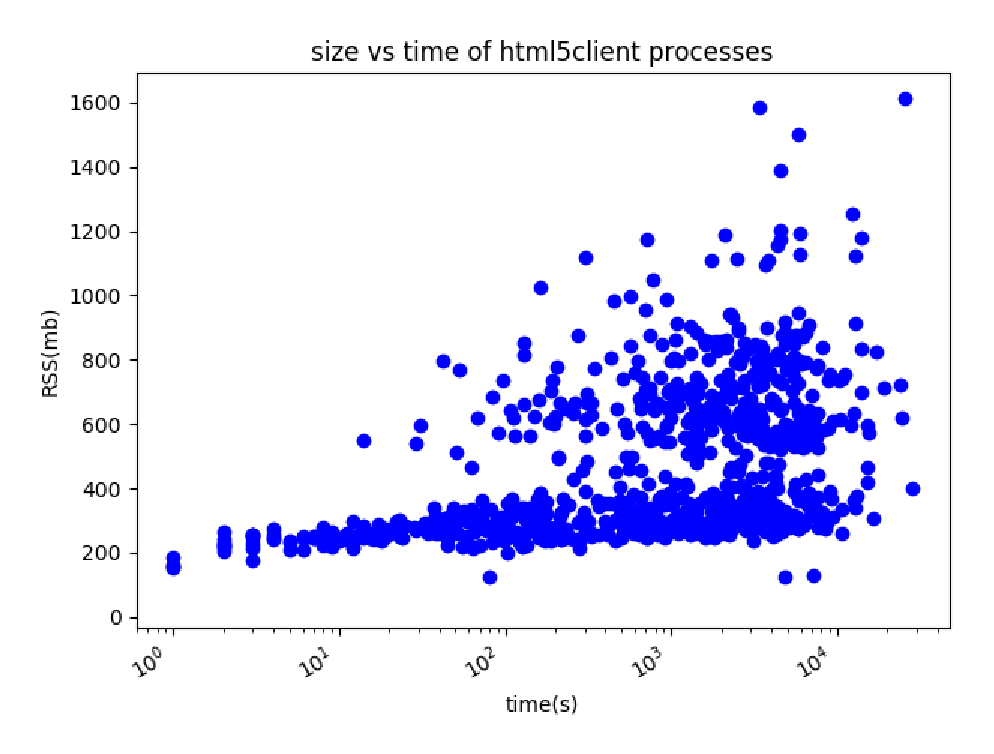
\includegraphics[width=\textwidth]
        {figures/211SizeVsTime}}
        \caption{\label{FIGURE-AV211SizeVsTime} Session size vs time in AV2.11. Note: logarithmic scale on X axis.}
\end{figure}

\begin{figure}[H]
        \center{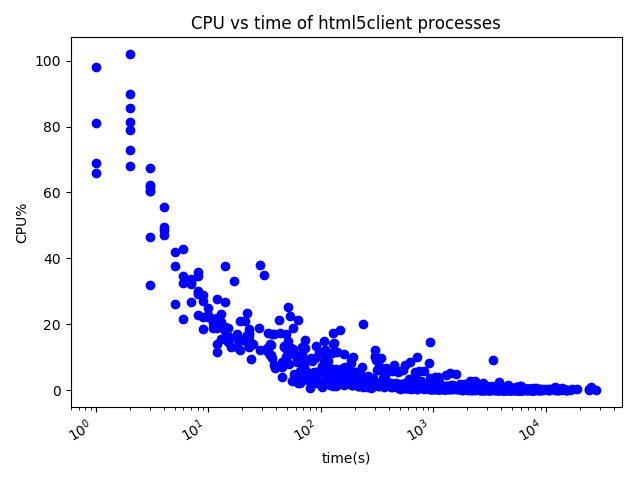
\includegraphics[width=\textwidth]
        {figures/211CPUVsTime}}
        \caption{\label{FIGURE-AV211CPUVsTime} Session CPU use vs time in AV2.11. Note: logarithmic scale on X axis.}
\end{figure}



\newpage

\section{Memory Consumption AV2.16}
\label{SECTION-216Memory}

The one html5client process from AV2.11 has been split up into three processes in AV2.16. Those three processes are html5client-v3, WebKitWebProces, and WebKitNetworkProcess. Use metrics for html5client-v3 can be seen in table~\ref{TABLE-AV216html5}, figure~\ref{FIGURE-AV216htmlSizeVsTime}, and figure~\ref{FIGURE-AV216htmlCPUVsTime}. Use metrics for WebKitWebProces can be seen in table~\ref{TABLE-AV216WebKitWeb}, figure~\ref{FIGURE-AV216WebKitWebSizeVsTime}, and figure~\ref{FIGURE-AV216WebKitWebCPUVsTime}. Use metrics for WebKitNetworkProcess can be seen in table~\ref{TABLE-AV216WebKitNet}, figure~\ref{FIGURE-AV216WebKitNetSizeVsTime}, and figure~\ref{FIGURE-AV216WebKitNetCPUVsTime}. All three of these processes contribute to session memory utalization. 



\begin{figure}[H]
        \center{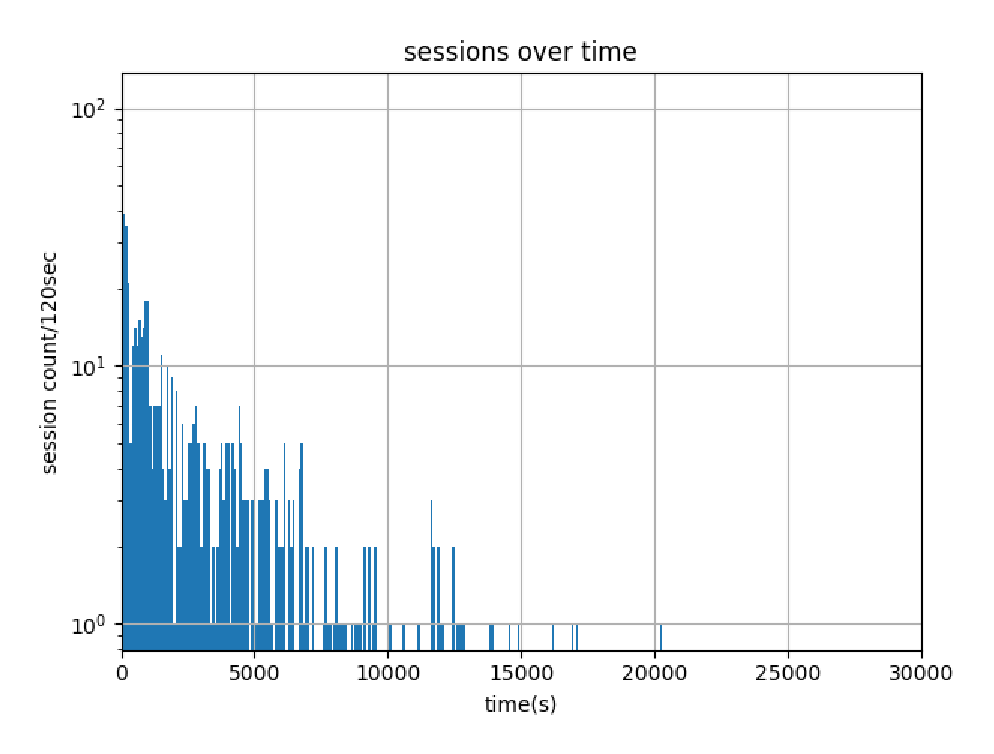
\includegraphics[width=\textwidth]
        {figures/216htmlSessionLength}}
        \caption{\label{FIGURE-AV216SessionLength} Histogram of session size over lifetime of session in AV2.16. Note: the 0-2min bin is not visible in this rendering, but there are 109 sessions under 2 min duration. Note: logarithmic scale on Y axis.}
\end{figure}



\begin{table}[H]
\begin{tabular}{|l|l|l|l|l|}
\hline BODCMA&                     ELAPSED&        CPU\%&     RSS(mb)&       SIZE(mb) \\
\hline count&                     647&  647&  647&     647 \\
\hline mean&   0 days 00:41:36&    0.722&   42.501&   91931.165 \\
\hline std&    0 days 00:53:23&    1.237&    8.033&    8377.031 \\
\hline min&           0 days 00:00:01&    0.000&   22.676&   84006.056 \\
\hline 25\%&           0 days 00:03:15&    0.000&   36.746&   84076.594 \\
\hline 50\%&           0 days 00:17:31&    0.200&   41.260&   84096.984 \\
\hline 75\%&           0 days 01:04:55&    0.900&   46.546&  100851.594 \\
\hline max&           0 days 05:38:21&   11.000&   68.404&  100884.672 \\
\hline 
\end{tabular}
\caption{\label{TABLE-AV216html5}Size of the html5client-v3 in AV2.16 from BODCMA on 12/11.} 
\end{table}



\begin{figure}[H]
        \center{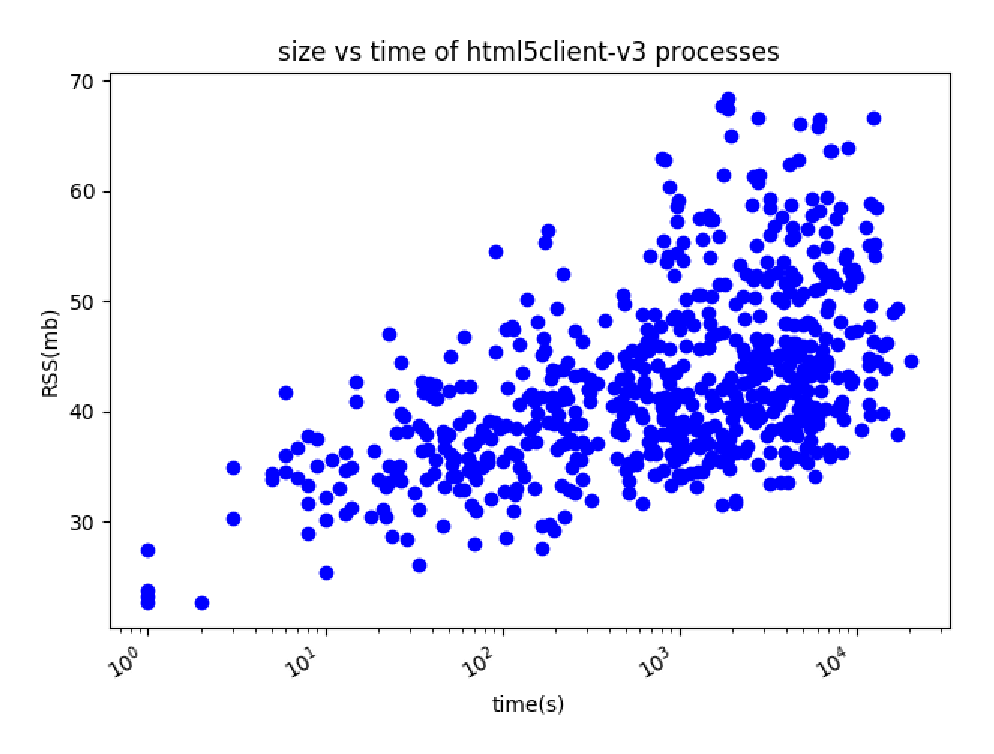
\includegraphics[width=\textwidth]
        {figures/216htmlSizeVsTime}}
        \caption{\label{FIGURE-AV216htmlSizeVsTime} Session size vs time for html5client-v3 process in AV2.16. Note: logarithmic scale on X axis.}
\end{figure}

\begin{figure}[H]
        \center{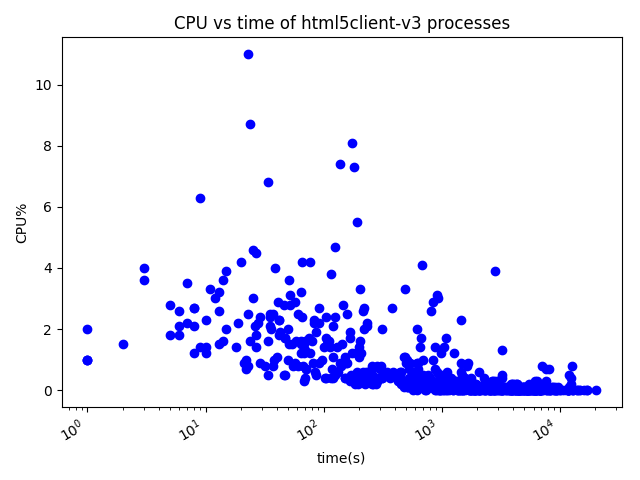
\includegraphics[width=\textwidth]
        {figures/216htmlCPUVsTime}}
        \caption{\label{FIGURE-AV216htmlCPUVsTime} Session CPU use vs time for html5client-v3 process in AV2.16. Note: logarithmic scale on X axis.}
\end{figure}



\begin{table}[H]
\begin{tabular}{|l|l|l|l|l|}
\hline BODCMA&                      ELAPSED&        CPU\%&     RSS(mb)&       SIZE(mb) \\
\hline count&                     656&  656&  656&     656 \\
\hline mean&   0 days 00:40:47&    5.752&  266.999&   93440.243 \\
\hline std&    0 days 00:53:18&   13.255&   82.332&    8393.289 \\
\hline min&           0 days 00:00:01&    0.100&   22.256&   84533.872 \\
\hline 25\%&           0 days 00:02:50&    0.400&  206.010&   85016.358 \\
\hline 50\%&    0 days 00:17:30&    1.000&  250.402&   86006.644 \\
\hline 75\%&    0 days 01:03:40&    5.000&  319.057&  101795.888 \\
\hline max&           0 days 05:39:13&  153.000&  979.200&  103066.800 \\
\hline 
\end{tabular}
\caption{\label{TABLE-AV216WebKitWeb}Size of the WebKitWebProces in AV2.16 from BODCMA on 12/11.} 
\end{table}



\begin{figure}[H]
        \center{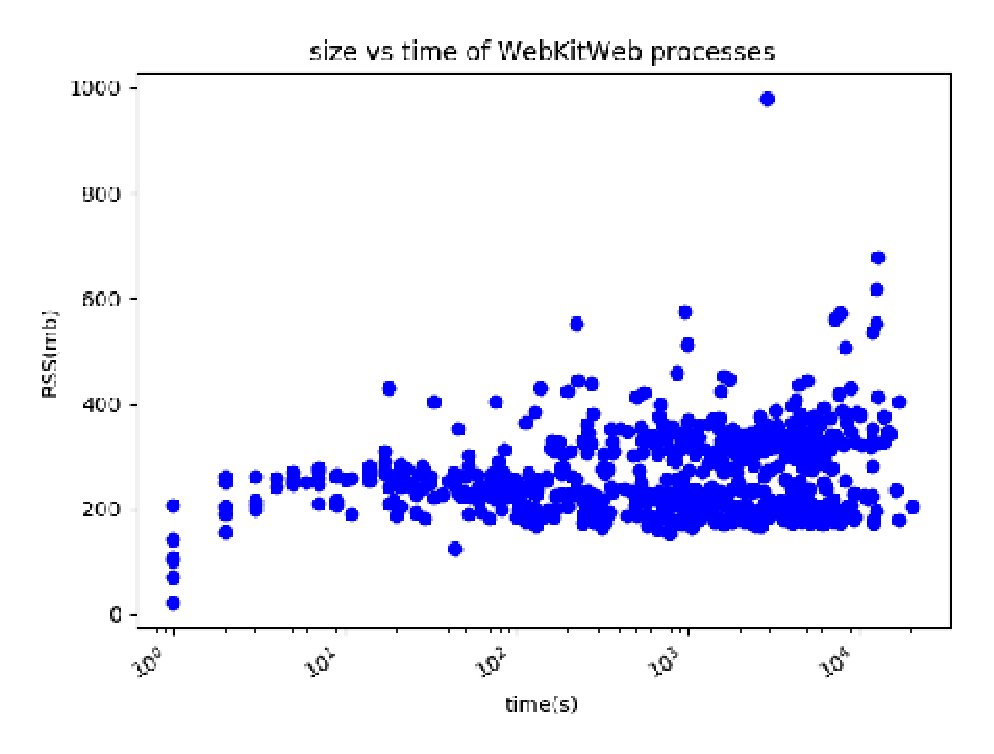
\includegraphics[width=\textwidth]
        {figures/216WebKitWebSizeVsTime}}
        \caption{\label{FIGURE-AV216WebKitWebSizeVsTime} Session size vs time for WebKitWebProces in AV2.16. Note: logarithmic scale on X axis.}
\end{figure}

\begin{figure}[H]
        \center{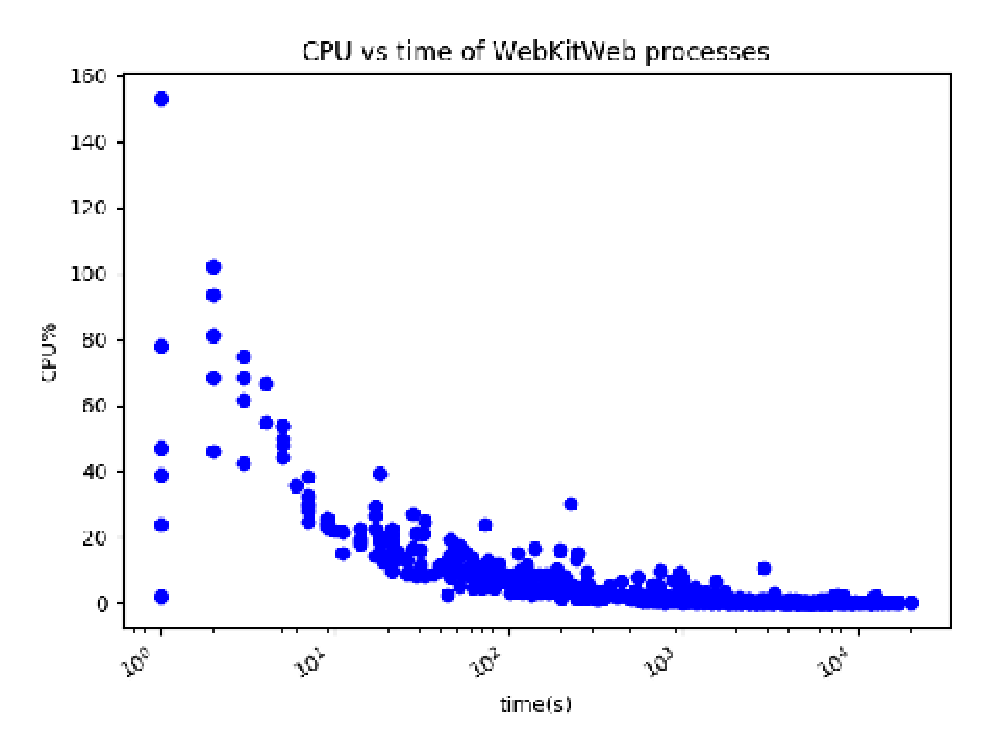
\includegraphics[width=\textwidth]
        {figures/216WebKitWebCPUVsTime}}
        \caption{\label{FIGURE-AV216WebKitWebCPUVsTime} Session CPU use vs time for WebKitWebProces in AV2.16. Note: logarithmic scale on X axis.}
\end{figure}



\begin{table}[H]
\begin{tabular}{|l|l|l|l|l|}
\hline BODCMA&                      ELAPSED&        CPU\%&     RSS(mb)&       SIZE(mb) \\
\hline count&                     650&  650&  650&     650 \\
\hline mean&   0 days 00:41:14&    0.384&   32.740&   92995.586 \\
\hline std&    0 days 00:53:34&    1.134&    1.725&    8394.076 \\
\hline min&           0 days 00:00:00&    0.000&   30.552&   84149.040 \\
\hline 25\% &          0 days 00:03:06&    0.000&   31.472&   84583.276 \\
\hline 50\%&           0 days 00:18:09&    0.000&   32.074&   92880.718 \\
\hline 75\%&    0 days 01:03:40&    0.200&   33.507&  101360.492 \\
\hline max&           0 days 05:40:03&    9.600&   41.704&  101549.928 \\
\hline 
\end{tabular}
\caption{\label{TABLE-AV216WebKitNet}Size of the WebKitNetworkProcess in AV2.16 from BODCMA on 12/11.} 
\end{table}



\begin{figure}[H]
        \center{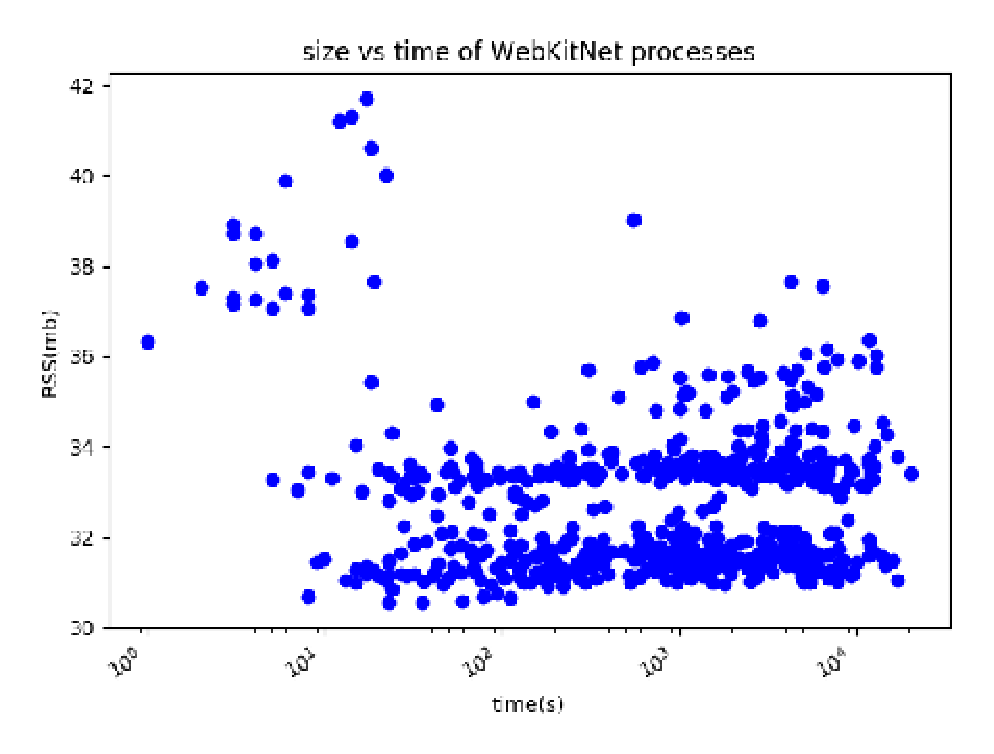
\includegraphics[width=\textwidth]
        {figures/216WebKitNetSizeVsTime}}
        \caption{\label{FIGURE-AV216WebKitNetSizeVsTime} Session size vs time for WebKitNetworkProcess in AV2.16. Note: logarithmic scale on X axis.}
\end{figure}

\begin{figure}[H]
        \center{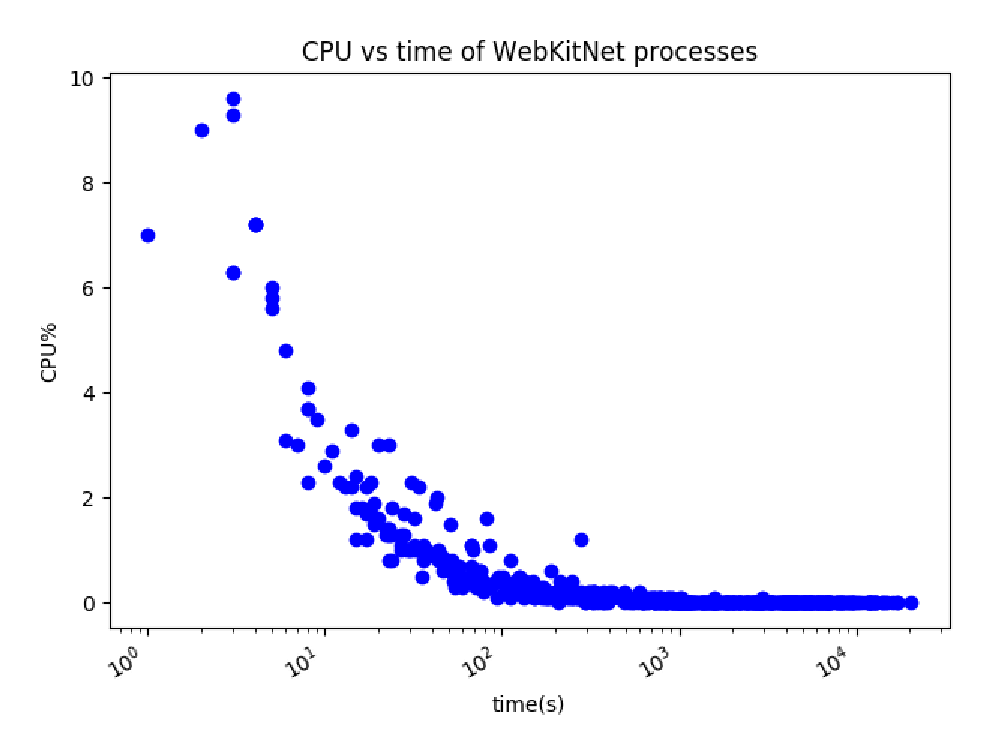
\includegraphics[width=\textwidth]
        {figures/216WebKitNetCPUVsTime}}
        \caption{\label{FIGURE-AV216WebKitNetCPUVsTime} Session CPU use vs time for WebKitNetworkProcess in AV2.16. Note: logarithmic scale on X axis.}
\end{figure}



By taking these three processes and combining them we can get a comparable result for session memory utalization. Each process's average utalization can be added, and their standard deviations can be added in quadrature to yield a meaningful result. The html5 process has RSS of $42 \pm 8$ MB, WebkitWeb $266 \pm 82$ MB, and WebKitNet $32 \pm 1$ MB. This gives an overall session RSS of $340 \pm 82$ MB. Because of the overallocation of memory by webkit-v3 a result for the VMS SIZE is not meaningful. This RSS measurement, by the nature of how RSS is reported, under-represents the actual memory used. One stitcher reported 18 sessions, which would correspond to 6.1GB of memory used, but in actuality the stitcher was using 14.8GB of memory reported by 'free -m'. The use of 'free -m revealed approx 7GB of shared libraries loaded into memory for that stitcher which is not included in the RSS session size reporting. Shared memory has significantly increased from AV2.11 to AV2.16, from approx 2GB up to 7GB per stitcher. The local ATS instance as well as other system processes account for the difference in total memory used compared to the 6.1GB memory used by sessions and the 7GB of memory in shared memory space used by SGUI. 



\section{Memory Use In QAM vs. DOCSIS}
\label{SECTION-QAMDOCSIS}

Memory utalization in AV2.11 is higher in QAM markets compared to DOCSIS, which is especially true for the largest sessions in QAM markets which have climbed up to 20GB of memory used for one session. This buildup of memory happens when users load large libraries. In webkit-v2 memory which was allocated was not properly deallocated by the garbage collector. In webkit-v3 the behaviour of the garbage collector changed, and memory is more aggressivly deallocated once it has fallen out of scope. This means that when libraries are loaded, they get removed once the user is done browsing those assets. QAM markets have shown higher max memory utalization by sessions, and this means larger gains in session size are expected in QAM markets compared to DOCSIS. Boston is a DOCSIS market which was not under imediate capacity constraint, and so larger savings in memory use are expected from the L-CHTR QAM markets. The exact gains which materialize there will be measured upon sucessful deployment of AV2.16 in a QAM market. 



\section{Conclusion}
\label{SECTION-Conclusion}

In AV2.11 average session size was reported as RSS $460 \pm 235$ MB and SIZE $744 \pm 356$ MB. This is in contrast to AV2.16 which is using RSS $340 \pm 82$ MB but is retaining significant shared memory allocations. RSS size has come down by 26\%, with a corresponding 65\% reduction in the standard deviation, but because of shared memory allocation which is not reported by RSS, and the over-allocation of VMS by webkit-v3, not all of these gains are realized. If we average out the shared memory by the number of sessions we can approximate the amount of shared memory which would be reported by VMS and make a comparison of memory use between the AV versions. With the example stitcher described in section~\ref{SECTION-216Memory}, 7GB of shared memory across 18 sessions corresponds to 388MB added memory per session. That shared memory averaged out across sessions and added to the 340MB average session size would yield an estimated use of memory (real and shared) of approx 728MB per session, which does not statistically differ from the average VMS memory usage of AV2.11. The reduction of RSS and the resulting decrease in the standard deviation of RSS which yielded overall gains in memory usage when compared to AV2.11 were mostly offset by increased use of shared memory, yielding little gains in overall stitcher memory usage in Boston. Further investigation into shared memory usage is needed to understand how shared memory increases and decreases with use patterns, and scales with session count. What gains in memory consumption were made were in the largest sessions, which from a preliminary measurement have gone down in size. The largest performance improvements are expected in the highest memory usage sessions, and those reside in L-CHTR QAM markets, so large gains were not expected in this market. Further investigation into performance in QAM markets will be nessicary to demonstrate if the change in webkit version has had the effect of reducing memory use for the largest sessions. 



\end{document}

